\documentclass{ximera}

%\usepackage{todonotes}

\newcommand{\todo}{}

\usepackage{esint} % for \oiint
\graphicspath{
  {./}
  {ximeraTutorial/}
}

\newcommand{\mooculus}{\textsf{\textbf{MOOC}\textnormal{\textsf{ULUS}}}}

\usepackage{tkz-euclide}
\tikzset{>=stealth} %% cool arrow head
\tikzset{shorten <>/.style={ shorten >=#1, shorten <=#1 } } %% allows shorter vectors

\usetikzlibrary{backgrounds} %% for boxes around graphs
\usetikzlibrary{shapes,positioning}  %% Clouds and stars
\usetikzlibrary{matrix} %% for matrix
\usepgfplotslibrary{polar} %% for polar plots
\usetkzobj{all}
\usepackage[makeroom]{cancel} %% for strike outs
%\usepackage{mathtools} %% for pretty underbrace % Breaks Ximera
\usepackage{multicol}
\usepackage{pgffor} %% required for integral for loops


%% http://tex.stackexchange.com/questions/66490/drawing-a-tikz-arc-specifying-the-center
%% Draws beach ball 
\tikzset{pics/carc/.style args={#1:#2:#3}{code={\draw[pic actions] (#1:#3) arc(#1:#2:#3);}}}



\usepackage{array}
\setlength{\extrarowheight}{+.1cm}   
\newdimen\digitwidth
\settowidth\digitwidth{9}
\def\divrule#1#2{
\noalign{\moveright#1\digitwidth
\vbox{\hrule width#2\digitwidth}}}





\newcommand{\RR}{\mathbb R}
\newcommand{\R}{\mathbb R}
\newcommand{\N}{\mathbb N}
\newcommand{\Z}{\mathbb Z}

\newcommand{\sagemath}{\textsf{SageMath}}


%\renewcommand{\d}{\,d\!}
\renewcommand{\d}{\mathop{}\!d}
\newcommand{\dd}[2][]{\frac{\d #1}{\d #2}}
\newcommand{\pp}[2][]{\frac{\partial #1}{\partial #2}}
\renewcommand{\l}{\ell}
\newcommand{\ddx}{\frac{d}{\d x}}

\newcommand{\zeroOverZero}{\ensuremath{\boldsymbol{\tfrac{0}{0}}}}
\newcommand{\inftyOverInfty}{\ensuremath{\boldsymbol{\tfrac{\infty}{\infty}}}}
\newcommand{\zeroOverInfty}{\ensuremath{\boldsymbol{\tfrac{0}{\infty}}}}
\newcommand{\zeroTimesInfty}{\ensuremath{\small\boldsymbol{0\cdot \infty}}}
\newcommand{\inftyMinusInfty}{\ensuremath{\small\boldsymbol{\infty - \infty}}}
\newcommand{\oneToInfty}{\ensuremath{\boldsymbol{1^\infty}}}
\newcommand{\zeroToZero}{\ensuremath{\boldsymbol{0^0}}}
\newcommand{\inftyToZero}{\ensuremath{\boldsymbol{\infty^0}}}



\newcommand{\numOverZero}{\ensuremath{\boldsymbol{\tfrac{\#}{0}}}}
\newcommand{\dfn}{\textbf}
%\newcommand{\unit}{\,\mathrm}
\newcommand{\unit}{\mathop{}\!\mathrm}
\newcommand{\eval}[1]{\bigg[ #1 \bigg]}
\newcommand{\seq}[1]{\left( #1 \right)}
\renewcommand{\epsilon}{\varepsilon}
\renewcommand{\phi}{\varphi}


\renewcommand{\iff}{\Leftrightarrow}

\DeclareMathOperator{\arccot}{arccot}
\DeclareMathOperator{\arcsec}{arcsec}
\DeclareMathOperator{\arccsc}{arccsc}
\DeclareMathOperator{\si}{Si}
\DeclareMathOperator{\proj}{\vec{proj}}
\DeclareMathOperator{\scal}{scal}
\DeclareMathOperator{\sign}{sign}


%% \newcommand{\tightoverset}[2]{% for arrow vec
%%   \mathop{#2}\limits^{\vbox to -.5ex{\kern-0.75ex\hbox{$#1$}\vss}}}
\newcommand{\arrowvec}{\overrightarrow}
%\renewcommand{\vec}[1]{\arrowvec{\mathbf{#1}}}
\renewcommand{\vec}{\mathbf}
\newcommand{\veci}{{\boldsymbol{\hat{\imath}}}}
\newcommand{\vecj}{{\boldsymbol{\hat{\jmath}}}}
\newcommand{\veck}{{\boldsymbol{\hat{k}}}}
\newcommand{\vecl}{\boldsymbol{\l}}
\newcommand{\uvec}[1]{\mathbf{\hat{#1}}}
\newcommand{\utan}{\mathbf{\hat{t}}}
\newcommand{\unormal}{\mathbf{\hat{n}}}
\newcommand{\ubinormal}{\mathbf{\hat{b}}}

\newcommand{\dotp}{\bullet}
\newcommand{\cross}{\boldsymbol\times}
\newcommand{\grad}{\boldsymbol\nabla}
\newcommand{\divergence}{\grad\dotp}
\newcommand{\curl}{\grad\cross}
%\DeclareMathOperator{\divergence}{divergence}
%\DeclareMathOperator{\curl}[1]{\grad\cross #1}
\newcommand{\lto}{\mathop{\longrightarrow\,}\limits}

\renewcommand{\bar}{\overline}

\colorlet{textColor}{black} 
\colorlet{background}{white}
\colorlet{penColor}{blue!50!black} % Color of a curve in a plot
\colorlet{penColor2}{red!50!black}% Color of a curve in a plot
\colorlet{penColor3}{red!50!blue} % Color of a curve in a plot
\colorlet{penColor4}{green!50!black} % Color of a curve in a plot
\colorlet{penColor5}{orange!80!black} % Color of a curve in a plot
\colorlet{penColor6}{yellow!70!black} % Color of a curve in a plot
\colorlet{fill1}{penColor!20} % Color of fill in a plot
\colorlet{fill2}{penColor2!20} % Color of fill in a plot
\colorlet{fillp}{fill1} % Color of positive area
\colorlet{filln}{penColor2!20} % Color of negative area
\colorlet{fill3}{penColor3!20} % Fill
\colorlet{fill4}{penColor4!20} % Fill
\colorlet{fill5}{penColor5!20} % Fill
\colorlet{gridColor}{gray!50} % Color of grid in a plot

\newcommand{\surfaceColor}{violet}
\newcommand{\surfaceColorTwo}{redyellow}
\newcommand{\sliceColor}{greenyellow}




\pgfmathdeclarefunction{gauss}{2}{% gives gaussian
  \pgfmathparse{1/(#2*sqrt(2*pi))*exp(-((x-#1)^2)/(2*#2^2))}%
}


%%%%%%%%%%%%%
%% Vectors
%%%%%%%%%%%%%

%% Simple horiz vectors
\renewcommand{\vector}[1]{\left\langle #1\right\rangle}


%% %% Complex Horiz Vectors with angle brackets
%% \makeatletter
%% \renewcommand{\vector}[2][ , ]{\left\langle%
%%   \def\nextitem{\def\nextitem{#1}}%
%%   \@for \el:=#2\do{\nextitem\el}\right\rangle%
%% }
%% \makeatother

%% %% Vertical Vectors
%% \def\vector#1{\begin{bmatrix}\vecListA#1,,\end{bmatrix}}
%% \def\vecListA#1,{\if,#1,\else #1\cr \expandafter \vecListA \fi}

%%%%%%%%%%%%%
%% End of vectors
%%%%%%%%%%%%%

%\newcommand{\fullwidth}{}
%\newcommand{\normalwidth}{}



%% makes a snazzy t-chart for evaluating functions
%\newenvironment{tchart}{\rowcolors{2}{}{background!90!textColor}\array}{\endarray}

%%This is to help with formatting on future title pages.
\newenvironment{sectionOutcomes}{}{} 



%% Flowchart stuff
%\tikzstyle{startstop} = [rectangle, rounded corners, minimum width=3cm, minimum height=1cm,text centered, draw=black]
%\tikzstyle{question} = [rectangle, minimum width=3cm, minimum height=1cm, text centered, draw=black]
%\tikzstyle{decision} = [trapezium, trapezium left angle=70, trapezium right angle=110, minimum width=3cm, minimum height=1cm, text centered, draw=black]
%\tikzstyle{question} = [rectangle, rounded corners, minimum width=3cm, minimum height=1cm,text centered, draw=black]
%\tikzstyle{process} = [rectangle, minimum width=3cm, minimum height=1cm, text centered, draw=black]
%\tikzstyle{decision} = [trapezium, trapezium left angle=70, trapezium right angle=110, minimum width=3cm, minimum height=1cm, text centered, draw=black]


\title{The Grocery Store}

\begin{document}

\begin{abstract}
%Stuff can go here later if we want!
\end{abstract}

\maketitle

\begin{sectionOutcomes}

After completing this section, students should understand relations and functions as mathematical tools. 

\begin{itemize}
\item Students .
\item Students .
\end{itemize}

\end{sectionOutcomes}





We run our daily lives by our understanding the connections between things.  There is no better example of this than the grocery store.  While shopping, we understand that there is a connection between products and prices. We often use this product-price relation to make shopping decisions.  Let's investigate this product-price relation.

Just like with NFL quarterbacks, this is a big relation with lots of pairs, too many pairs.  We'll simplify a bit to make it more manageable. 

\begin{itemize}
\item We'll focus on a single store : Bob's Groceries
\item We'll focus on a single day : Aug 12, 2015
\end{itemize}


\begin{definition}
\textbf{The Product-Price Relation}
\begin{itemize}
\item The domain of the Product-Price Relation is the collection of all products in Bob's Groceries on Aug 12, 2015. 
\item The codomain of the Product-Price Relation is the collection of all prices. 
\item A (product, price) pair is in the Product-Price Relation if this product had this price in Bob's Groceries on Aug 12, 2015. Otherwise, it is not in the Product-Price Relation.
\end{itemize}
\end{definition}


\quad \\



\begin{example}
\begin{itemize}
\item (Freshair Wheat Bread, \$1.19) $\in$ Product-Price
\item (Greenforest Yellow Corn, \$0.89) $\in$ Product-Price
\item (Greenforest Yellow Corn, \$0.79) $\in$ Product-Price
 \end{itemize}
 \end{example}


\quad \\




\textbf{More Simplifying} 

It is possible that there is more than one size of Greenforest Yellow Corn, which could add some confusion.  Instead of writing a description of the product, let?s use the global trade identification number, i.e. its bar code number.


\begin{definition}
\textbf{The Product-Price Relation (improved)}
\begin{itemize}
\item The domain of the Product-Price Relation is the collection of all product GTIN numbers used in Bob's Groceries on Aug 12, 2015. 
\item The codomain of the Product-Price Relation is the collection of all prices. 
\item A (number, price) pair is in the Product-Price Relation if this is a GTIN number for a product in Bob's Groceries and this product had this price in Bob's Groceries on Aug 12, 2015. Otherwise, it is not in the Product-Price Relation.
\end{itemize}
\end{definition}



\begin{example}
\begin{itemize}
\item (145526374467, \$1.19) $\in$ Product-Price
\item (176228354233, \$0.89) $\in$ Product-Price
\item (176228354233, \$0.79) $\in$ Product-Price
 \end{itemize}
 \end{example}

\quad \\

\textbf{Product-Price}
To the right are all of the pairs inside the Product-Price relation.  Bob's Grocery is not a very big store. (It scrolls.)
A list is one mathematical tool for describing the connections in this relation.

\[
\begin{array}{|l|l|l|}
\hline
(102707849467, 1.24) & (151603090297, 1.28) & (147882057258, 1.33) \\\hline
(121219574901, 3.95) & (196997564303, 4.61) & (120984686834, 1.39) \\\hline
(192107524489, 3.06) & (116532522722, 5.46) & (190132246907, 1.24) \\\hline
(105853328761, 1.33) & (185066339518, 1.25) & (178355581117, 4.81) \\\hline 
(139647551818, 0.79) & (182604889507, 2.07) & (163639788196, 0.95) \\\hline 
(151593345667, 2.07) & (173630558604, 1.24) & (141821520319, 1.25) \\\hline 
(142144767669, 3.38) & (187266863018, 2.63) & (146494777598, 1.33) \\\hline 
(155152532584, 3.06) & (159664504967, 0.79) & (137707844901, 3.67) \\\hline 
(116506724164, 2.17) & (139411323037, 1.71) & (127419334209, 1.90) \\\hline 
(120957405055, 4.66) & (133860480889, 1.39) & (145242561846, 0.79) \\\hline 
(105756538007, 0.95) & (162440197320, 1.46) & (198053092474, 1.39) \\\hline 
(130874077288, 1.39) & (136348437875, 2.46) & (147817810438, 4.66) \\\hline 
(133727371104, 0.79) & (182108962832, 6.79) & (158625940456, 2.68) \\\hline 
(100883301040, 3.07) & (103811801019, 2.07) & (185611457154, 3.06) \\\hline 
(184348593986, 1.33) & (135757760868, 2.40) & (187006291505, 3.38) \\\hline 
(143404118258, 5.94) & (185248264403, 0.79) & (116047586435, 1.39) \\\hline 
(189778504216, 1.25) & (187266173278, 1.66) &    \\\hline
\end{array}
\]



Another tool is a picture map.
\begin{image}
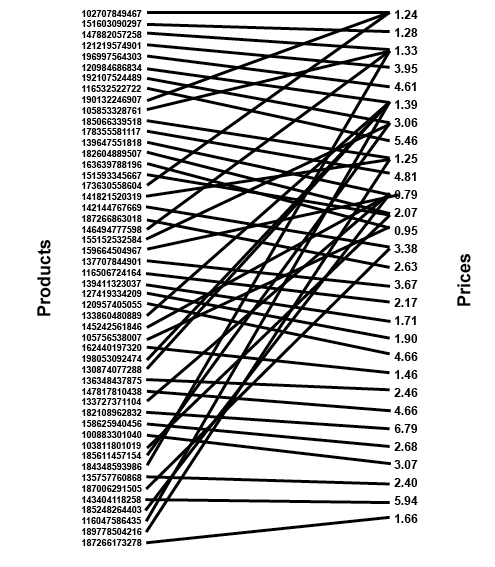
\includegraphics{pics/Product_Price_Map.png}
\end{image}

The map lists the domain items and the codomain items and then identifies pairs in the relation with a line segment.



GTIN numbers are twelve digit numbers, but not every twelve digit number is a GTIN number. That means not every twelve digit number is in the domain the Product-Price relation.

It could also happen that the twelve digit number is a GTIN number, but Bob?s Groceries might not carry that product.  Again the number would not be in the domain.

This will be a common theme with our functions. By describing the domain as GTIN numbers we know that we are dealing with 12-digit numbers, but not all 12-digit numbers. Our description is implying which 12-digit numbers are in the domain.  We say that the domain is implied.

\begin{definition}
An implied domain is one that is not stated explicitly. It is inferred from the description of the relation.
\end{definition}













\end{document}
